% Slides for 2025-07-29
% To create a slide, use the following:
% \begin{frame}{TITLE}
%     BODY
% \end{frame}

% To create a slide with a bullet list, use the following:
% \begin{frame}{TITLE}
%     \begin{itemize}
%         \item ITEM 1
%         \item ITEM 2
%     \end{itemize}    
% \end{frame}

% To create a slide with numbered list, use the following:
% \begin{frame}{TITLE}
%     \begin{enumerate}
%         \item ITEM 1
%         \item ITEM 2
%     \end{enumerate}
% \end{frame}

% To create a slide with a graphic:
% 1. Add the graphic to this folder (named picture.png)
% 2. Use the following:
% \begin{frame}{TITLE}
%     \centering
%     \includegraphics[height=0.7\textheight,width=0.7\textwidth,keepaspectratio]{picture.png}
% \end{frame}

% To create a slide with two columns, use the following:
% \begin{frame}{TITLE}
%     \begin{columns}
%         \begin{column}{0.5\textwidth}
%             COLUMN 1 BODY
%         \end{column}
%         \begin{column}{0.5\textwidth}
%             COLUMN 2 BODY
%         \end{column}
%     \end{columns}
% \end{frame}

% DO NOT DELETE MY SLIDE - BRENDON!!!!
\begin{frame}{FishSense Mobile Android}
    \vfill
    \centering
    \begin{columns}
        % Column 1: Camera Image
        \begin{column}{0.32\textwidth}
            \centering
            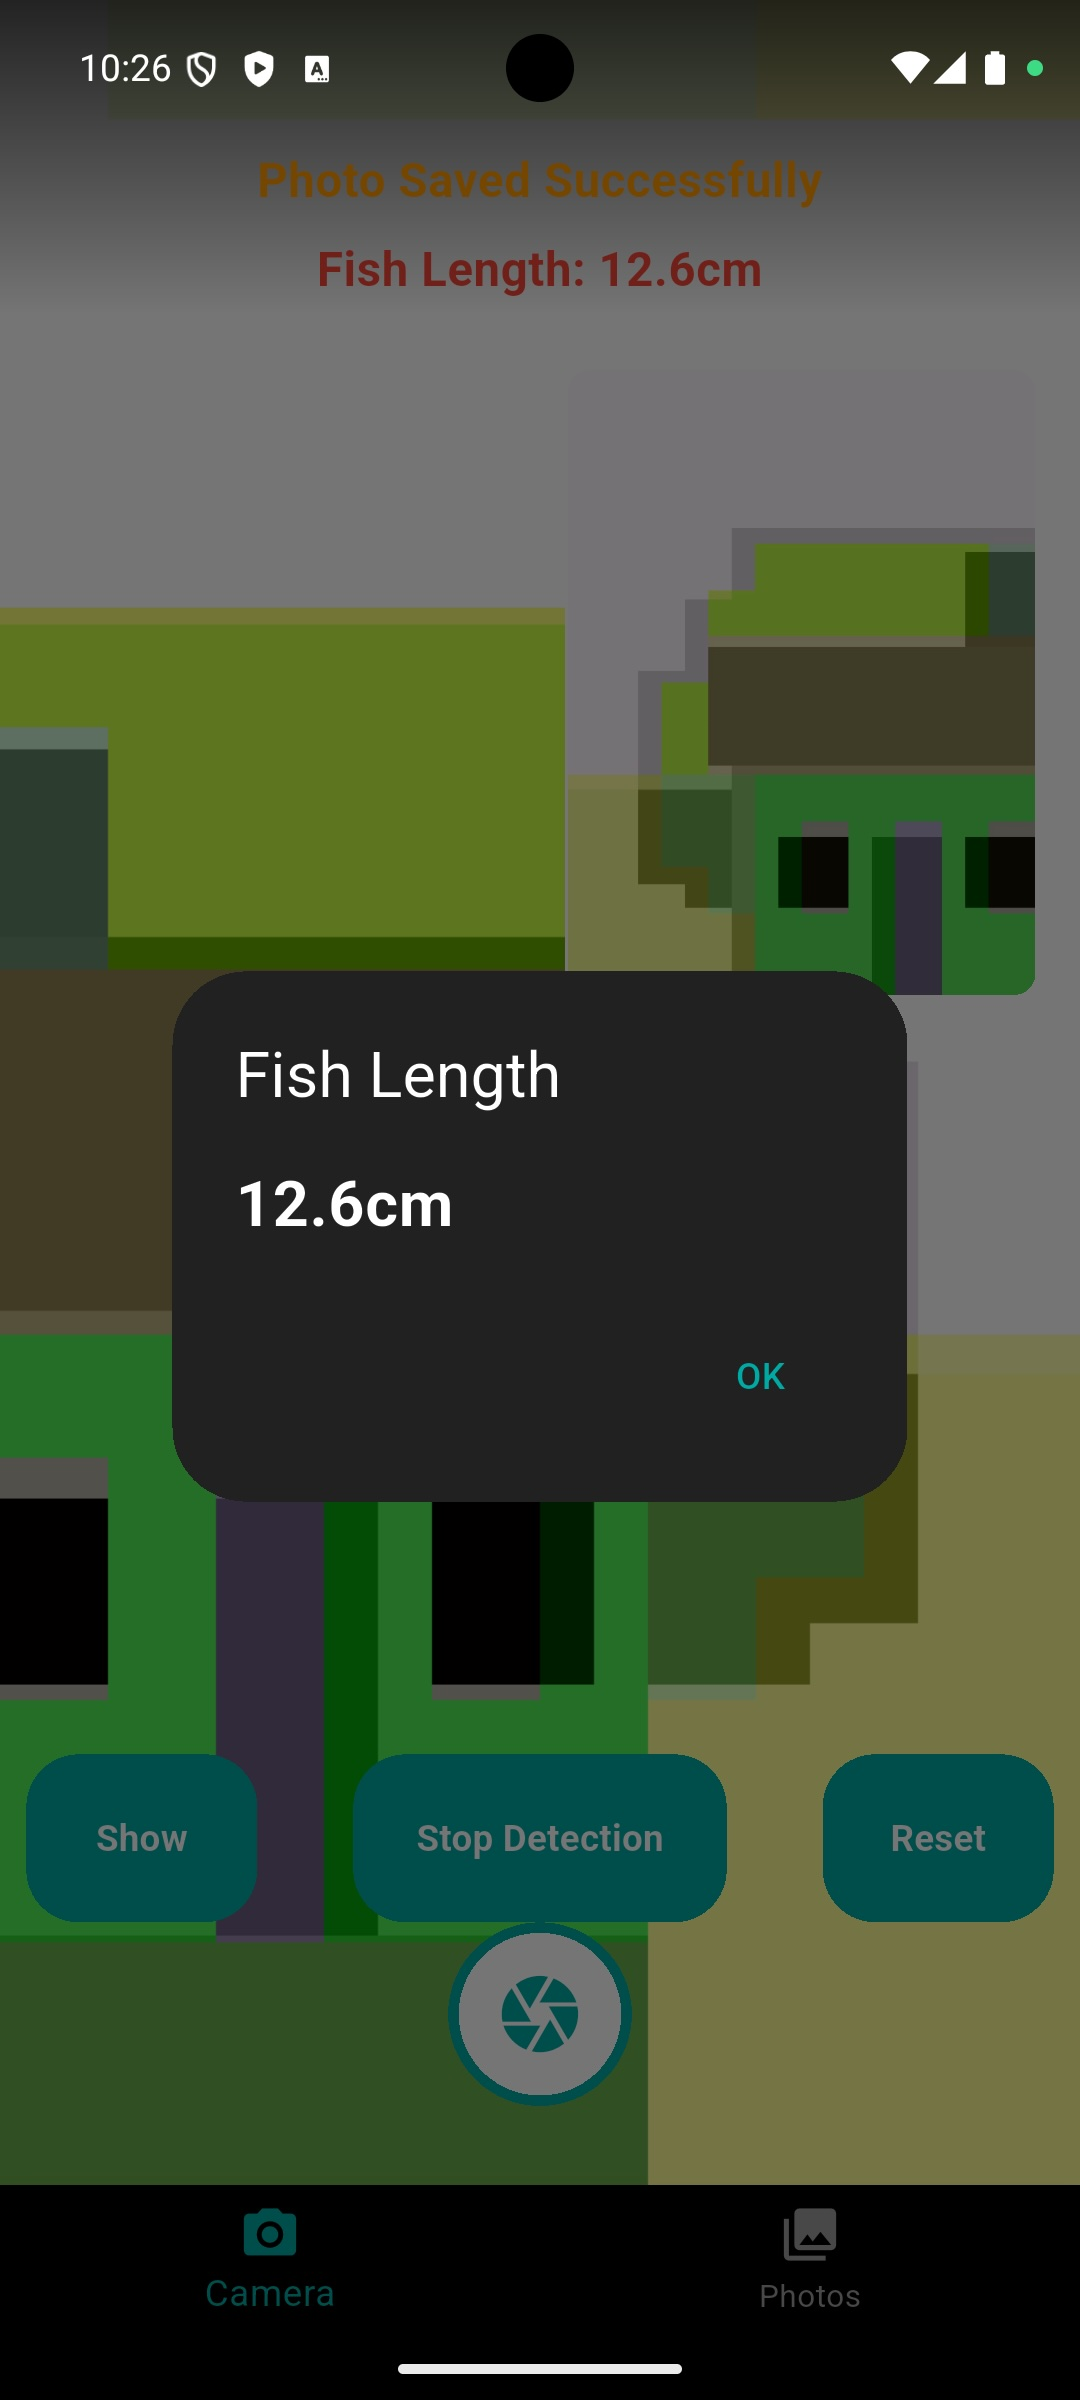
\includegraphics[height=0.8\textheight,keepaspectratio]{images/CameraImage.jpg}
            
            \vspace{0.2cm}
            \textbf{Current Progress:} \\
            Camera with Mock Data
        \end{column}
        
        % Column 2: Gallery Image
        \begin{column}{0.32\textwidth}
            \centering
            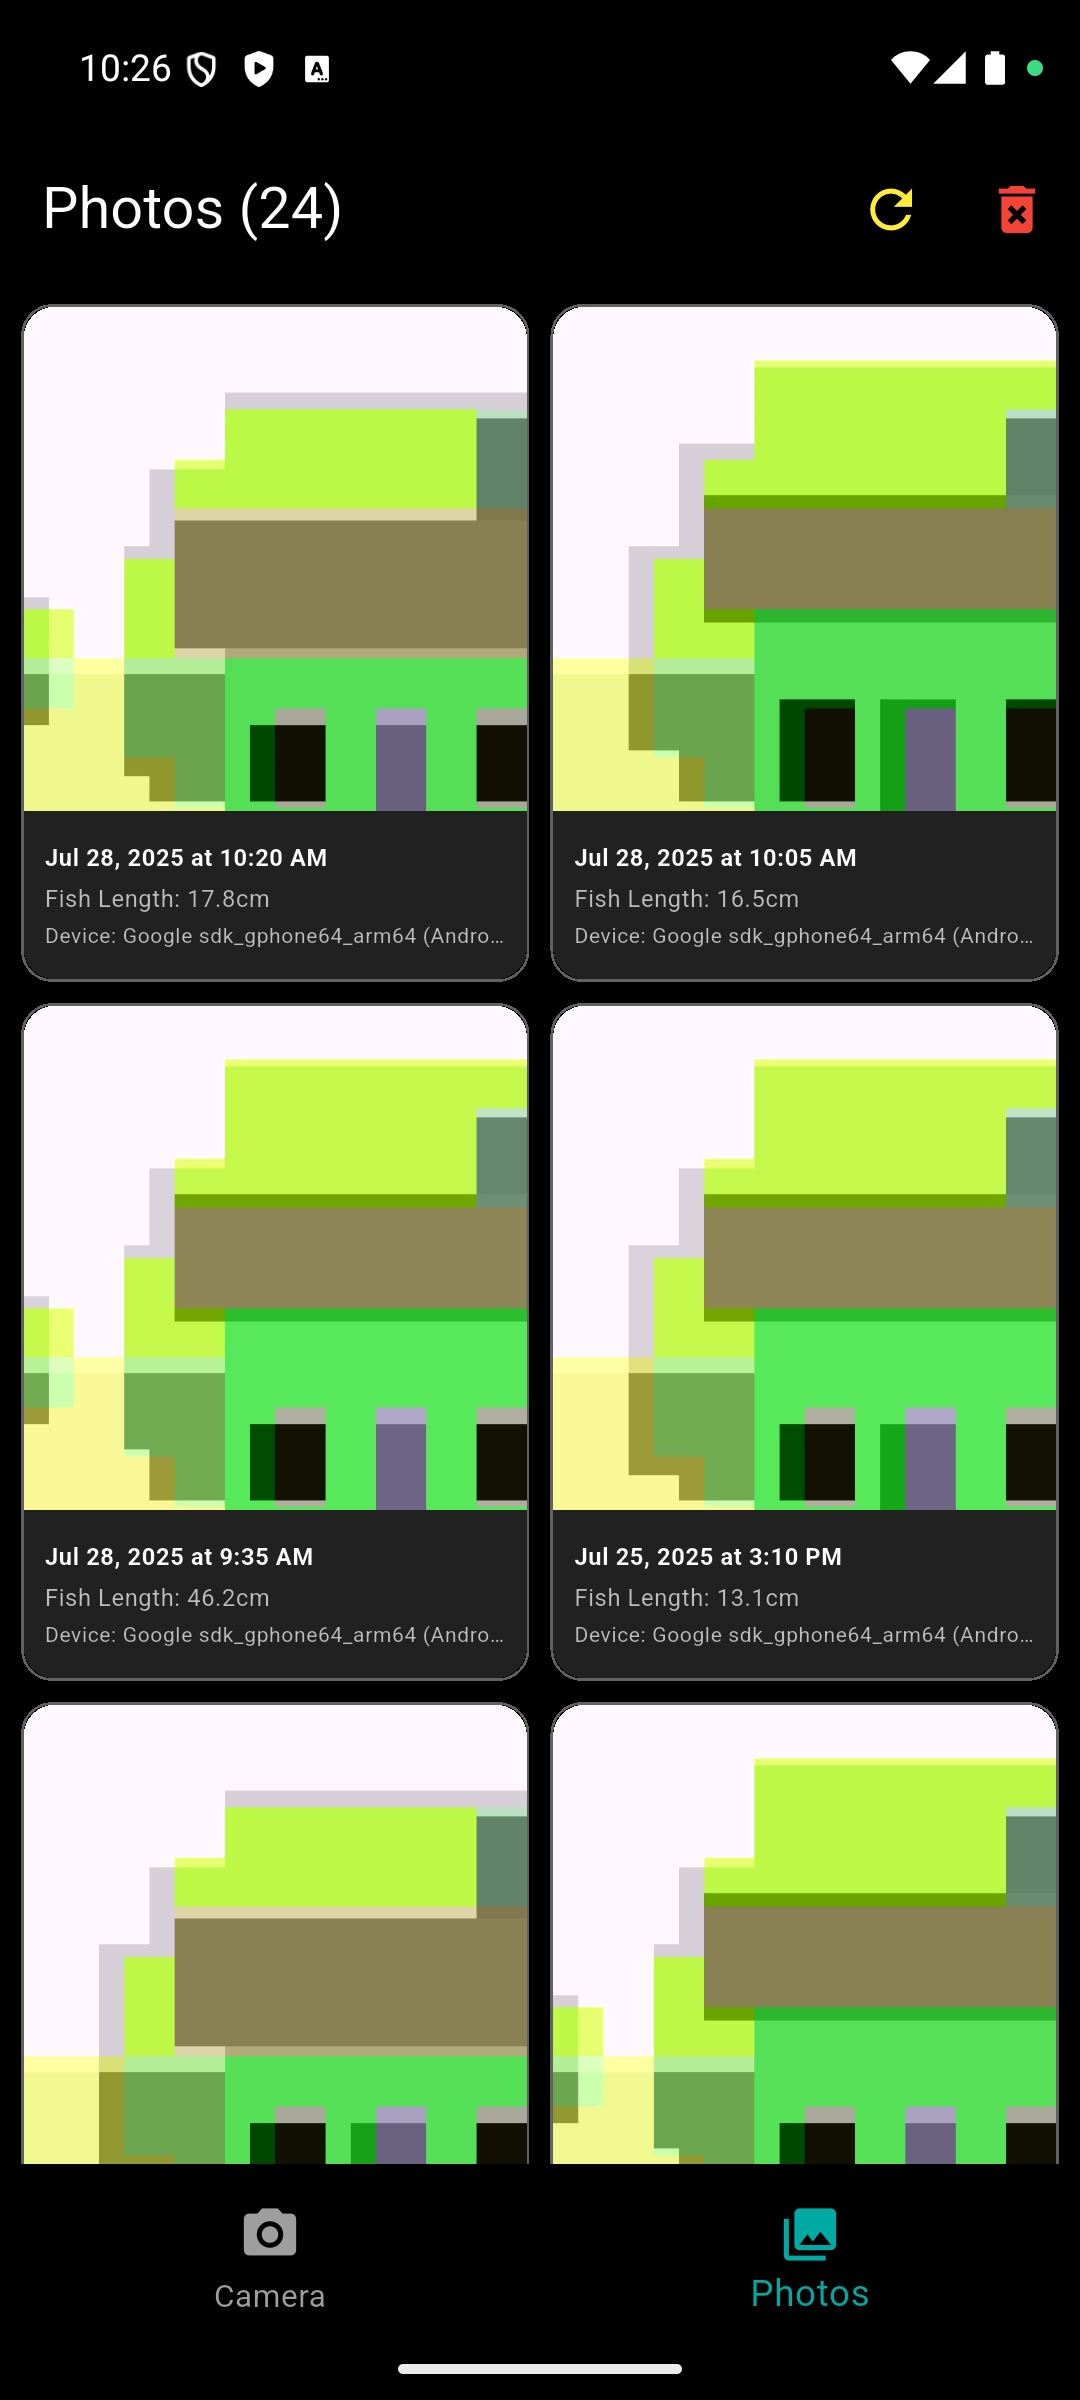
\includegraphics[height=0.8\textheight,keepaspectratio]{images/GalleryImage.jpg}
            
            \vspace{0.2cm}
            \textbf{Current Progress:} \\
            Gallery with Mock Data
        \end{column}
        
        % Column 3: Diagram Image
        \begin{column}{0.32\textwidth}
            \centering
            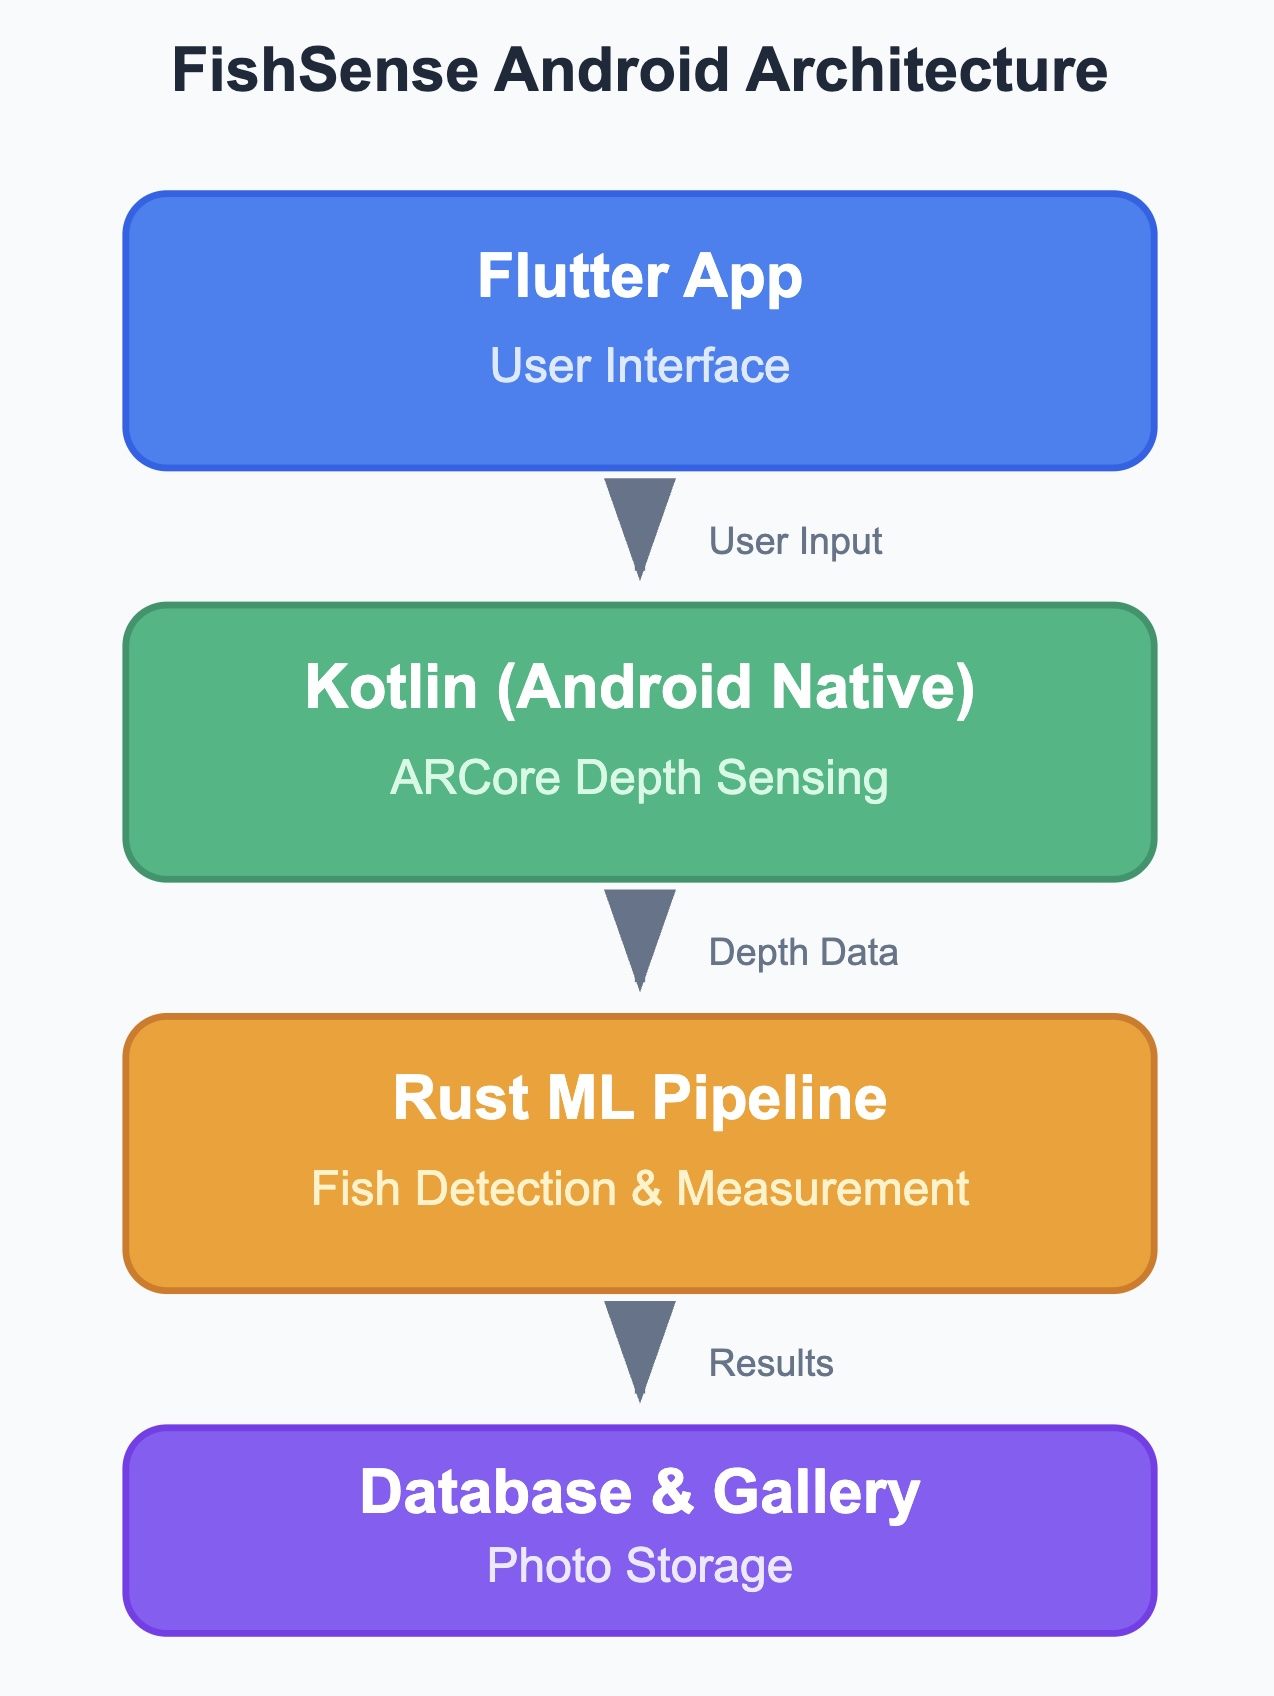
\includegraphics[height=0.7\textheight,keepaspectratio]{images/Diagram1.jpg}
            
            \vspace{0.1cm}
            \textbf{Next Steps:} \\
            ARCore Integration
        \end{column}
    \end{columns}
    \vfill
\end{frame}

